% Setup - do not change
\documentclass[11pt]{article}
\usepackage[top=0.9in, left=0.9in, bottom=0.9in, right=0.9in]{geometry} 
\usepackage{parskip}

\usepackage[english]{babel}
\usepackage[utf8]{inputenc}
\usepackage{amsmath,amsthm,amssymb,graphicx,pdfpages,lipsum,hyperref}
\usepackage[none]{hyphenat}
\usepackage{csquotes}

\setlength\parindent{0pt}
%%%%%%%%%%%%%%%%%%%%%%%%%%%%%%%%%%%%%%%%%%%%%%%%%%%%%%%%%%%%%%%%%%%
% add other packages here if required
\usepackage{graphicx}
\usepackage{subcaption} % For subfigures
\usepackage{hyperref}
\usepackage{float}

%% Bibliography are specified in this file. You can also choose inline bib style if you want to. But make sure your citation style is consistent (and proper)
% For more details on citation: https://library.unimelb.edu.au/recite
\usepackage[sorting = none]{biblatex}
\addbibresource{references.bib}

%%%%%%%%%%%%%%%%%%%%%%%%%%%%%%%%%%%%%%%%%%%%%%%%%%%%%%%%%%%%%%%%%%% the '%' symbol denotes comments

% Begin document creation
% DELETE THE \lipsum PLACEHOLDERS WHEN YOU BEGIN
\title{\textbf{Investigating the Effects of Shootings on Taxi Demand in New York City}}
\author{
Harry Fisher \\
Student ID: 1082897 \\
%% Replace the link with your github repo
% 1. Remember to escape underscore (\_) in the link.
% 2. Remember to include the commit you want to submit in the link
\href{https://github.com/MAST30034-Applied-Data-Science/mast30034-project-1-HFISHER00/commit/ced29bbf7fd3b989f2876ecc9c600d9fccb8a563}{Github repo with commit}
}
\begin{document}
\maketitle

\section{Introduction}
% Link to a 30 min tutorial if you require revision: https://www.overleaf.com/learn/latex/Learn_LaTeX_in_30_minutes

\hspace{0pt}Gun violence in the United States has always been a major concern. The rise of COVID and the introduction of lockdowns caused civil unrest, increasing the issue. Notably, New York City (NYC) shootings’ have increased since 2020 (Sarasa-Cabezuelo, 2023). This report aims to investigate the relationship between the demand for taxis in NYC, and the public’s perception of safety post-shootings. The hypothesis is that the public think their safety after shootings will be diminished. It is thought that taxi demand will decrease following a shooting. People might prefer to stay inside and stay safe rather than continue on with their regular way of living. 

Because of the increase in shootings in NYC since the pandemic, this report will utilise two different machine learning models to try and predict the hourly taxi demand in NYC from regular trips to those trips that occur within a week of a shooting in the same location.

Yellow taxis are the majority cab in NYC. They are generally owned by cab companies who lease the cars to their drivers who get to keep all of their fairs (Bryant, 2023). They are also the only vehicles allowed to pick up customers anywhere in the city (Hill, 2022). The findings of this report will benefit both the individual drivers of yellow cabs and the taxi companies too. By providing insights into demands after shootings, the outcomes might help change decisions on where taxis are deployed after shootings.

In this report, the demand for taxi rides will be represented by the number of pickups that occur within a location every hour. Changes in the hourly taxi trips will be able to show if there is a difference in demand.

\subsection{Dataset}

\hspace{0pt}The primary data set for this report is the TLC Yellow Taxi Trip Record Data created by the NYC Taxi and Limousine Commission. This dataset represents trip records from all those conducted by yellow taxis in NYC. This report assumed that records after 2020 would have been strongly impacted by Covid. Therefore, the data was restricted to Jan 2016 until December 2019 for analysis and modelling. This timeframe encapsulates a period before the disruptions caused by the pandemic. This was done to create a more accurate depiction of the city’s pre-pandemic operations, which is the assumed way of life that society wish to return to in the future.

\clearpage

To be used alongside the taxi trip data, the external NYPD Shooting Incident Data (Historic) published by the New York Police Department (NYPD) has also been integrated. This dataset ranges from 2006 to the 2023. This dataset has also been restricted to between Jan 2016 and December 2019 so analysis can be conducted on the effects of shootings in NYC. The dataset contains detailed information about the shootings, including the date, location, and people involved. This dataset was selected as it is expected that shootings will affect the demand for taxis. 

\begin{table}[htbp]
\centering
\begin{tabular}{|c|c|c|}
\hline
\textbf{Datasets} & \textbf{Number of Features} & \textbf{Number of Instances} \\
\hline
TLC Yellow Taxi Trip Records (2016-2019) & 19 & 432,101,963 \\
NYPD Shooting Incident Data (Historic) & 21 & 27,312 \\
\hline
\end{tabular}
\caption{The shape of both datasets used in this report.}
\end{table}

\section{Preprocessing}
\subsection{Data Cleaning}
\subsubsection{TLC Yellow Taxi Trip Record Data}
\hspace{0pt}The TLC Yellow Taxi Trip Record Data utilised spanned across a 4 year period. An in-depth inspection of the data found there cleaning of the data was required to ensure integrity, so meaningful analysis could be conducted. Several steps were taken to reduce inconsistencies and streamline the dataset. A major issue was to address nonsensical errors, so ranges were established for various features. This was helpful to fix any anomalies that were created either through not being entered, or being entered incorrectly. 

\begin{itemize} 
    \item Trips that had fares below the base rate of \$2.50 were deemed invalid and so were discarded. This value corresponds to the starting cost of all cab fares.
    \item Trips that were not allocated to a Location ID within the range of 1 to 263 were discarded. This is because values outside of that did not correspond to valid locations, warranting their exclusion. 
    \item Trips that were incorrectly recorded and had a drop-off time before the pickup time were discarded, ensuring the time-related aspect of the data kept its integrity.
    \item Trips that had less than 1 passenger were discarded as taxis only process fares when passengers are on board. This ensured that only relevant records were retained for analysis.  
\end{itemize} 

\hspace{0pt}The cleaning of the data found a total 11,137,747 entries that were erroneous and would effect the analysis. These instances were discarded. This left 420,964,216 trip records remaining, providing a robust foundation for future models.

\subsubsection{NYPD Shooting Incident Data (Historic)}
\hspace{0pt}The initial import of the shooting data contained 27,312 instances. The first step was to restrict the date range to align with the taxi trip data. This range was from the start of 2016 until the end of 2019. This restriction left the dataset with 4,103 instances. 

No further cleaning were required as all the important features were adequately completed. Any incomplete features in the dataset were deemed as unnecessary for the models being developed, meaning that instances with incomplete information could be retained.

\subsection{Feature Selection}
\subsubsection{TLC Yellow Taxi Trip Record Data}
\hspace{0pt}After cleaning the data, only certain features were retained from the to be used for further analysis. These were: ‘tpep\_pickup\_datetime’, ‘PULocationID’. These were retained as these are the only features that are known before a trip's occurrence that relate directly to demand, and so will be useful when predicting future demand. Feature engineering will be used to create extract other meaningful features.

\subsubsection{NYPD Shooting Incident Data (Historic)}
\hspace{0pt}The features retained were 'ID', 'Date', 'Latitude', and 'Longitude'. These features pair contain time-related and geospatial data. They can be used for predictive modelling and geospatial analysis alongside the taxi data.

\subsection{Feature Engineering and Dataframe Creation}
\hspace{0pt}For the taxi trip data, new features were engineered to extract further insights. Specifically, ‘Date’, ‘Hour’, and ‘Month’ attributes were created from the timestamp of the pickups. Additionally, an indicator was made to identify trips that occurred on weekends. These all are valuable features that could potentially be correlated with taxi demand. 

For the shooting data, the ‘Date’ column was used to create a ‘Date\_7\_days\_after’ feature to reveal the date a week after the initial shooting occurred. Another feature that was created was  ‘LocationID’ which was created from the Latitude and Longitude of the shooting data. This Location ID corresponds to the taxi zone the shooting occurred in.

In order to identify trips that occurred within a week of a shooting at the identical location, the shooting and taxi data frames were merged. Every shooting was matched with taxi trips that were picked up at the location of the shooting within the week of the occurrence. Within this dataframe, an additional feature, ‘days\_after\_shooting’, was engineered. This feature reveals the number of days that have passed after the shooting when that taxi trip took place. The idea behind this was the rationale that the taxi demand might fluctuate in the days after the shooting occurred. After an initial reduction, there could be a slow return to the regular demands as the days pass. 

\subsection{Aggregation and Last of Preprocessing}
\hspace{0pt}The merged data frame then underwent aggregation, organised by three features: Hour, days\_after\_shooting, and ID (of shooting). The aim was to compute and create a feature representing the number of trips conducted per hour in the same location of the shooting after it occurred. This was done as the aim of this investigation is identify if there is a change in demand after a shooting occurs. The size of the dataset after aggregation was 305,482

The original yellow taxi data frame also went underwent the same aggregation. This was done so a comparison could be made between regular time taxi demands and demands after a shooting. The size of this dataset after aggregation was 4,344,263.

After aggregation, and with the new feature of trips per hour, outliers were identified. Looking at the range of both the merged and regular taxi trips after aggregation, it was revealed that both had maximums values that exceeded 3,000 trips within a single hour, figures that seemed disproportionate to the normal trip patterns in the city. While the presence of major events could justify those instances, they were removed to create a more realistic range. The cut-off threshold was based on a Z-score of 3, leading to the removal of 1.6\% of hourly data instances.  The size of the hourly trips after shootings was then 300,549 and the size of the hourly trips at normal times was 4,240,679.

The last step of preprocessing involved the use of one-hot, whicd encoded categorical variables represented as numerical values. LocationID, Hours and Month columns were all one hot encoded, to create features that will effectively meet that needs of the learning models that will be utilised.

\section{Preliminary Analysis}
\hspace{0pt}The initial approach to this investigation involved averaging the hourly pick-ups that occurred on each of the 7 days and compare this to the hourly average for the whole of NYC. However, this initial thought does not adequately explain the entirety of the situation. Examining Figure 1 shows distinct disparities in the geographic distribution of pickups and shootings. They have ‘hotspots’ that are in different locations. Predominantly, areas like airports and Manahattan, the richest part of NYC often characterised by higher tourism (The Most Expensive Neighborhoods in NYC, 2023), contribute to the majority of taxi trips. In contrast, shooting incidents are concentrated in lower socioeconomic regions and particularly prominent in Brooklyn whereas are less common in wealthier regions like Manhattan. 

For example, a shooting could occur in Manhattan and lower the taxi demand. It is a busy area though so a large amount of taxi trips would still occur in the week after. On the other hand though if a shooting were to occur in a less busy spot in Brooklyn, the impact might be different. There could still be fewer trips but the effect might be the less obvious in a busier place like Manhattan.

\begin{figure}[htbp]
    \centering
    \begin{subfigure}[b]{0.48\textwidth}
        \centering
        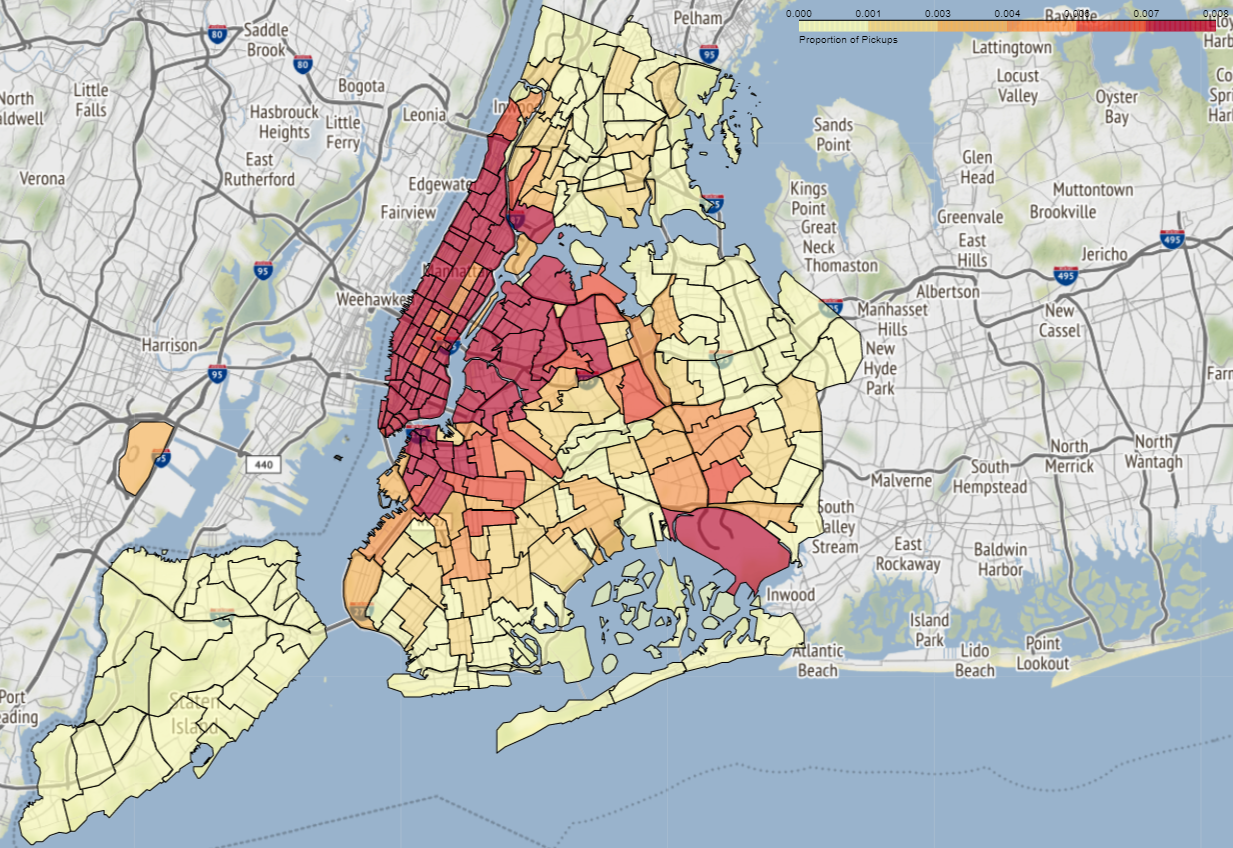
\includegraphics[width=\textwidth]{GeoVis Taxi.png}
        \caption{Taxi Pickups.}
        \label{fig:taxi}
    \end{subfigure}\hfill
    \begin{subfigure}[b]{0.48\textwidth}
        \centering
        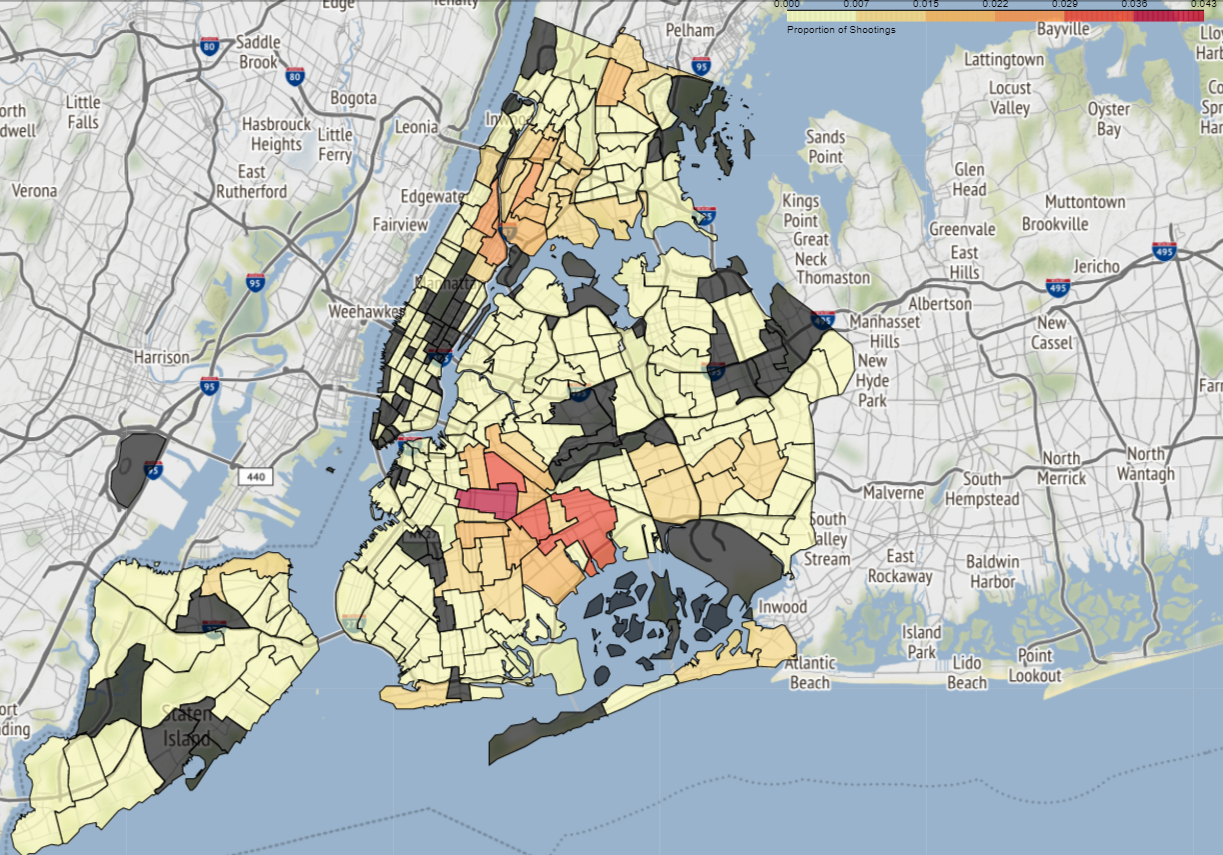
\includegraphics[width=\textwidth]{GeoVis Shooting.png}
        \caption{Shooting Occurrences.}
        \label{fig:shooting}
    \end{subfigure}
    \caption{Proportions of taxi trips (a) and shootings (b) in NYC.}
    \label{fig:both}
\end{figure}

\hspace{0pt}Consequently, a straight comparison of the averages will be insufficient. A different approach is required to identify effects shootings may have on taxi demand. Comparisons must be made specific to locations. Figure 2 does this and illustrates the average difference in trip numbers before and after a shooting occurrence, exclusively in the same location. The plot reveals a reduction in trips where the shooting occurred during the following week. This supports the hypothesis that shootings do have an effect on taxi demand. 

\hspace{0pt}Another thought was that average hourly trips would increase back to regular demand in a few days after shootings. Figure 3 dispels that idea, showing that there is no change in demands within the first week after a shooting. This observation meant the attention of the report remained on the effects of a shooting on taxi trips on the whole week proceeding. 

\begin{figure}[htbp]
    \centering
    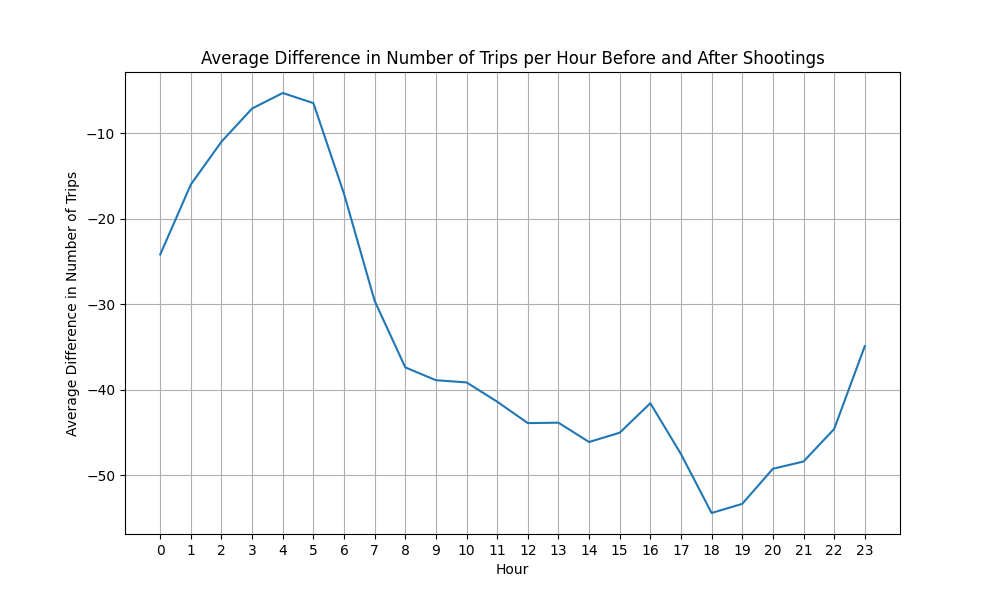
\includegraphics[width=0.8\textwidth]{shooting_hourly_effects_plot.png}
    \caption{Average difference in number of trips occurring at the location of shooting for hour before and after. Hour is time of day.}
    \label{fig:taxi}
\end{figure}

\begin{figure}[H]
    \centering
    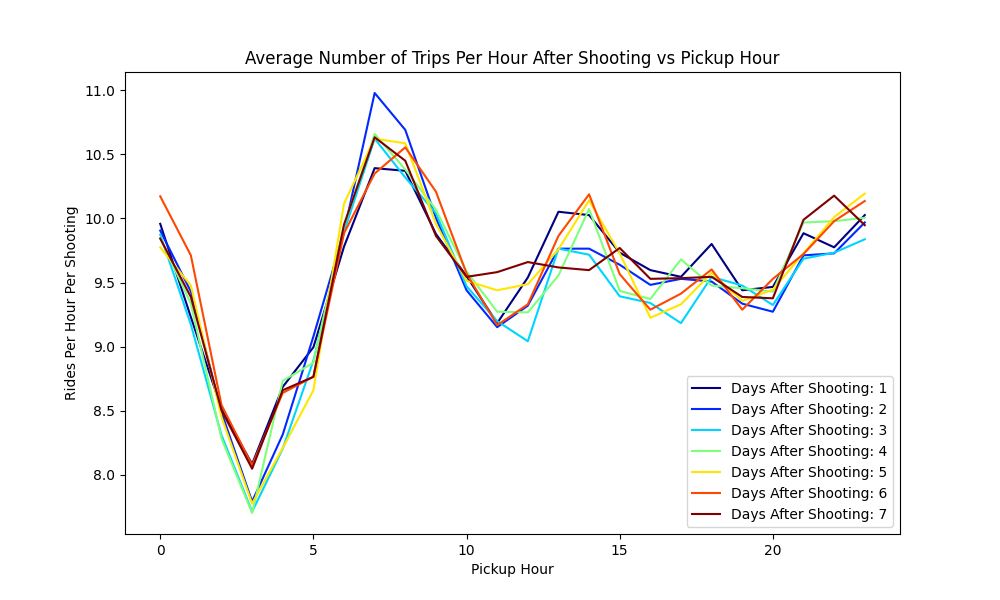
\includegraphics[width=0.8\textwidth]{Daily_Avg_Trips_Post_Shooting.png}
    \caption{Average number of trips for week after shooting in the same location.}
    \label{fig:taxi}
\end{figure}

\section{Modelling}
\hspace{0pt}Two different regression models were used to predict hourly taxi demands in NYC. Regression models were chosen as a result of the target variable, trips per hour, which comprises of continuous numerical data. This made classification models unsuitable. The models chosen were Support Vector Regression (SVR) and Linear Regression. 

Both the shooting-related trips and regular taxi trips were merged to train the models. To identify if a trip occurred within one week of a shooting, a new binary column ‘Shooting’ was created. The years 2016-2018 were used as the training set, with the 2019 year used as the testing set. This is close to the 80-20 split that is very common when splitting the data into training and testing sets. It's pertinent to note that no cross-validation was conducted in this study.

\subsection{Support Vector Regression(SVR)}
\hspace{0pt}SVR, similar to Support Vector Machines (SVM), depends on the idea of creating a regression line or hyperplane to optimally fit the data. SVM differs, as it functions as a classifier, using a hyperplane to separate the data into distinct classes. SVR is trained using a symmetrical loss function, which equally penalises high and low estimates (Awad \& Khanna, 2015, p. 67). This characteristic proves useful in the context of this investigation, to make predictions on hourly pickups. This model assumed there was independence between variables, which is reasonable as none of the variables (time, location or shooting) are associated with each other. SVR is also suitable as the categorical predictor variables have been one-hot encoded. This is beneficial as it avoids any incorrect ordinal assumptions. 

\subsection{Linear Regression}
\hspace{0pt}Linear Regression relates predictor variables with the target variable. The aim is to understand the underlying linear relationships between them (Lederer, 2021, p. 38). The same assumptions for SVR apply to Linear Regression. 

\section{Results and Discussion}
\hspace{0pt}To evaluate both models, both Root Mean Squared Error (RMSE) and R-Squared (R2) metrics were used. These values allow valuable interpretations into different aspects of the models’ predictive accuracy and goodness of fit. RMSE is easily understandable, representing the average difference in trips per hour between the prediction and observation. R2 is a little less interpretable but still significant. It represents the amount of variance in the observed taxi data that can be explained by the predictors of the models.

Table 2 shows that both SVR and Linear Regression performed similarly, shown by their RMSE and R2 values. The marginal difference between the models reveals the comparability between SVR and Linear Regression. 

\begin{table}[htbp]
    \centering
    \begin{tabular}{lcc}
        \hline
        Model & RMSE & R2 \\
        \hline
        SVR & 68.68 & 0.6420 \\
        Linear Regression & 67.56 & 0.6419 \\
        \hline
    \end{tabular}
    \caption{Comparison of Model Performance}
    \label{tab:model_comparison}
\end{table}

Looking at RMSE in isolation, both models seemed to be performing rather poorly. An average RMSE exceeding 65 suggests the models have limited practical use, considering the range for the hourly taxi data is [1, 610] (after removal of outliers). 

However, the inspection of R2 provides a different perspective. The values are both above 0.6, suggesting the models explain a substantial amount of the data’s variability. Looking at Figure 4, it can also be seen that although the predictions are substantially different to the actual data, the trends are very similar.

The issues with the results could have occurred for a few different reasons. The models might have overfitted the noise in the training set, not learning the underlying pattern of the dataa, and so do not generalise well to new data. The training data might have not been diverse enough, and so the models lack robustness and fail to generalise.

\begin{figure}[htbp]
    \centering
    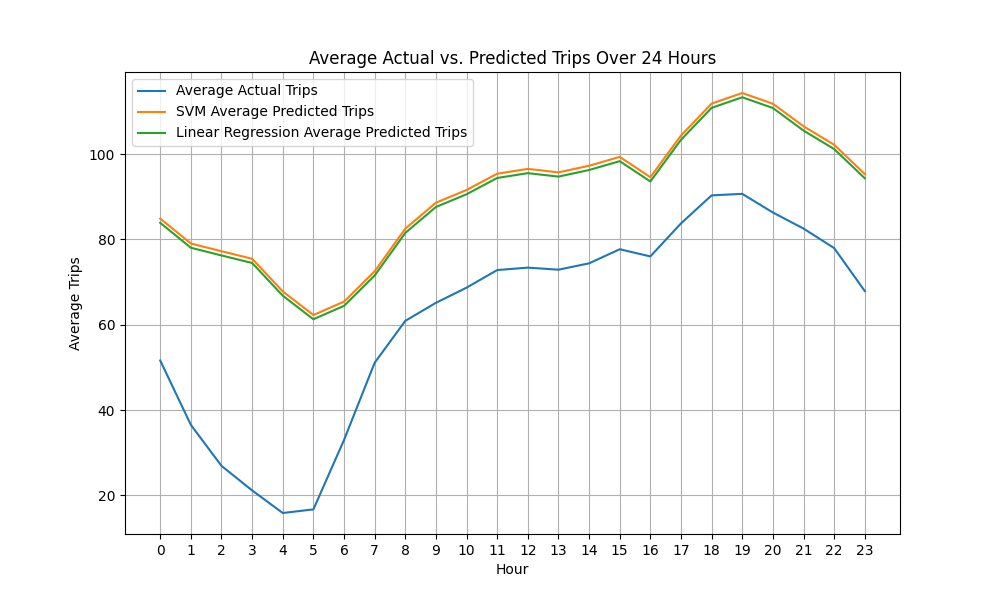
\includegraphics[width=0.8\textwidth]{Model_Results_plot.png}
    \caption{Model predictions compared to actual hourly trips.}
    \label{fig:taxi}
\end{figure}

Investigating the feature importance in Table 3 reveals some interesting results. Surprisingly, location seemed to not effect the model, while hour, month and shooting occurrences all played a similarly equal role in the predictions. Weekends caused a slight increase in taxi demands. The most notable value though is that shootings occurrences resulted in a reduction in number of trips per hour. 

 Overall, the SVR and Linear regression models in their current form cannot be used to insightful predictions. The results have shown though that shootings appear to result in a reduction of taxi demand. 

\begin{table}[htbp]
    \centering
    \begin{tabular}{lcc}
        \hline
        & SVR & Linear Regression \\
        \hline
        Hour\_encoded & -245.93 & -247.38 \\
        Month\_encoded & -237.27 & -238.72 \\
        Shooting & -234.48 & -235.94 \\
        Weekend & 1.74 & 1.75 \\
        LocationID\_encoded & 0.0 & 0.0 \\
        \hline
    \end{tabular}
    \caption{Feature Importance between SVR and Linear Regression}
    \label{tab:coefficients_comparison}
\end{table}

\section{Recommendations}
\hspace{0pt}Based on the evaluations of the models and their outcomes, it can be seen that their predictive capability  in estimating the hourly number of taxi trips (demand) for trips occurring within NYC is limited. With RMSE values greater than 60, these models have an average prediction error of 60 trips per hour. This clearly shows that they are not good at predicting the exact number of taxi trips per hour.

The R-Squared results do provide some interest, however. Both models have values above 0.6, meaning that they do capture some of the patterns and variability of the real-world data.

While an immediate course of action for yellow taxi companies is not recommended this study does highlight a notable finding. Shootings do effect the demand for taxis in NYC. Therefore, it is recommended that yellow companies investigate further into this issue. Because of these indications, investing resources into constructing a more accurate and generalisable model could prove valuable for optimising their operations.

In the interim, while further investigations occur, there is an actionable recommendation for yellow taxi drivers with autonomy over their stationing locations. The analysis clearly shows that the week following a shooting results in a reduction in trip demand. Because of this, it would be smart of the drivers to avoid stationing themselves at locations where shootings have occurred for at least a week. This strategy will help drivers meet the demands in alternate areas, optimising the driver’s driving time and resulting in more trips and hopefully more income for them. 

\section{Conclusion}
\hspace{0pt}This report investigated two different regression models that looked to predict hourly taxi demand in NYC. Using the NYPD’s shooting dataset in conjunction and TLC’s Yellow Taxi dataset, the effect of shootings on the demand was looked at. However, both the SVR and Linear Regression models performed underwhelmingly, failing to capture the intricacies of the data. 

Following this report, it might be worth considering further investigation into this matter. The introduction of more features, other external datasets, and the use of other models might help to find more informative and accurate  predictions.

In summary, this investigation helps to understand the interplay with shootings and taxi demand. While the initial models exhibit limitations, they lay the groundwork for future study in the area. It will help pave the way for further research in this domain.

\clearpage

% BEGIN REFERENCES SECTION
\printbibliography
\begin{thebibliography}{9}
\bibitem{awad}
Awad, M., \& Khanna, R. (2015). Efficient Learning Machines: Theories, Concepts, and Applications for Engineers and System Designers (p. 67). Apressopen.

\bibitem{bryant}
Bryant, S. (2023, February 27). How NYC’s Yellow Cab Works and Makes Money. Investopedia. \url{https://www.investopedia.com/articles/professionals/092515/how-nycs-yellow-cab-works-and-makes-money.asp}

\bibitem{hill}
Hill, K. (2022, January 16). What’s the Difference Between Green Cabs, Yellow Cabs \& Other Taxis in NYC? - CitySignal. CitySignal. \url{https://www.citysignal.com/whats-the-difference-between-green-cabs-yellow-cabs-other-taxis-in-nyc/}

\bibitem{lederer}
Lederer, J. (2021). Fundamentals of High-Dimensional Statistics (p. 38). Springer Nature.

\bibitem{nypd_shooting}
NYPD Shooting Incident Data (Historic) | NYC Open Data. (2023, April 28). Data.cityofnewyork.us. \url{https://data.cityofnewyork.us/Public-Safety/NYPD-Shooting-Incident-Data-Historic-/833y-fsy8}

\bibitem{sarasa}
Sarasa-Cabezuelo, A. (2023). Analysis of Gun Crimes in New York City. MDPI, 5(2), 1–21. \url{https://doi.org/10.3390}

\bibitem{propertyclub}
The Most Expensive Neighborhoods in NYC. (2023, May 1). PropertyClub. \url{https://propertyclub.nyc/article/most-expensive-neighborhoods-in-nyc\#:~:text=NYC\%20Real\%20Estate\%20Median\%20Sales\%20Prices\&text=Manhattan\%20has\%20the\%20most\%20expensive}

\bibitem{tlc_data}
TLC Trip Record Data - TLC. (2023, May). Www.nyc.gov. \url{https://www.nyc.gov/site/tlc/about/tlc-trip-record-data.page}


\end{thebibliography}


\end{document}